\section{Petri Nets}
\subsection{Modeling with Petri Nets}
\begin{exercise}{1}
Given the following process description, model it using a Petri net:
\begin{quote}
    A small bank has 3 employees to serve customers, each can only serve 1 customer at the same time.
    Due to space limitations, only 20 customers can be in the bank at the same time.
    After being served a customer can decide to queue again for
    another service.
\end{quote}
\end{exercise}
\paragraph{Solution:}
The Petri net can be modeled as follows:
\begin{figure}[H]
    \centering
    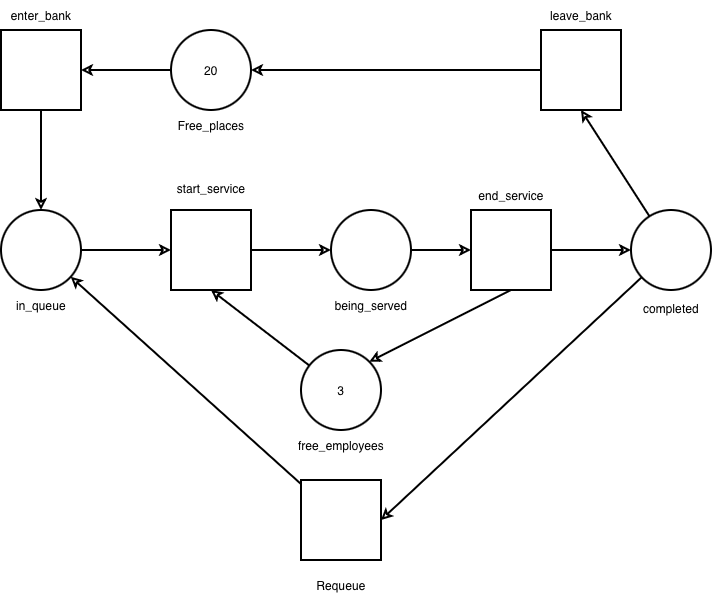
\includegraphics[width=0.7\textwidth]{images/exercises/petri_nets/petri_net-1.png}
    \caption{Petri Net Model of the Bank Process}
\end{figure}
Wee can see that:
\begin{itemize}
    \item To model the availability of employees, we use a place \(p_{\text{free\textunderscore employees}}\) with 3 tokens, representing the 3 available employees;
    \item To start serving a customer, both a token in \(p_{\text{free\textunderscore employees}}\) and a token in \(p_{\text{in\textunderscore queue}}\) are required;
    \item After being served, a token is added back to \(p_{\text{free\textunderscore employees}}\), representing the employee becoming free again;
    \item After being served, a customer can decide to queue again, represented by the loop back to \(p_{\text{in\textunderscore queue}}\) or to leave the bank, adding one token to \(p_{\text{free\textunderscore places}}\);
    \item To model the space limitation, we use a place \(p_{\text{free\textunderscore places}}\) with 20 tokens, representing the maximum number of customers allowed in the bank;
\end{itemize}
\subsection{Petri Net Properties}
\begin{exercise}{1}
Given the following Petri net:
\begin{figure}[H]
    \centering
    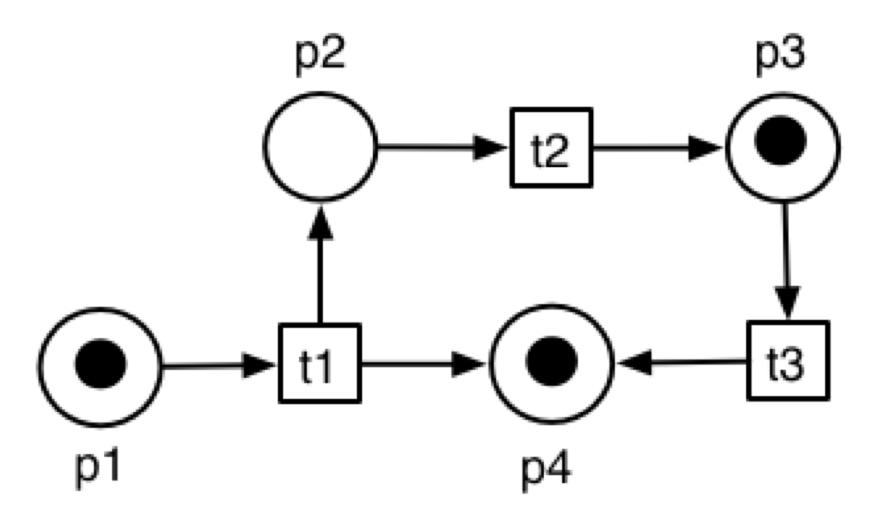
\includegraphics[width=0.5\textwidth]{images/exercises/petri_nets/petri_net-2.png}
\end{figure}
The exercise requires to:
\begin{enumerate}
    \item Formalize the Petri net as a tuple \(PN = (P, T, F, M_0)\);
    \item Define the preset and postset of each transition;
    \item Find the enabled transitions in the initial marking \(M_0\);
    \item Draw the reachability graph of the Petri net;
    \item Find the reachable terminal markings;
    \item Is there a reachable marking where we have a non-deterministic choice between two transitions? 
\end{enumerate}
\end{exercise}
\paragraph{Solution:}
\begin{enumerate}
    \item To formalize the Petri net, we need to define the sets of places, transitions, flow relations (esdges) and the initial marking:
    \begin{itemize}
        \item \(P = \{p_1, p_2, p_3, p_4\}\)
        \item \(T = \{t_1, t_2, t_3\}\)
        \item \(F = \{(p_1, t_1), (t_1, p_2), (t_1, p_4), (p_2, t_2), (t_2, p_3), (p_3, t_3), (t_3, p_4)\}\)
        \item The initial marking \(M_0\) is given by the tokens in the places at the start:
        \[M_0(p_1) = 1, M_0(p_2) = 0, M_0(p_3) = 0, M_0(p_4) = 0\]
    \end{itemize}
    \item To find the preset and postset of each transition, we look at the incoming and outgoing edges of each transition:
    \begin{itemize}
        \item \( \bullet t_1 = \{p_1\} \)
        \item \( t_1 \bullet = \{p_2, p_4\} \)
        \item \( \bullet t_2 = \{p_2\} \)
        \item \( t_2 \bullet = \{p_3\} \)
        \item \( \bullet t_3 = \{p_3\} \)
        \item \( t_3 \bullet = \{p_4\} \)
    \end{itemize}
    \item In the initial marking \(M_0\), we can clearly see that the that the enabled transition (have all the required tokens in its preset) are:
    \[ \text{Enabled transitions in } M_0: \{t_1, t_3\} \]
    \item The reachability graph can be constructed by firing the enabled transitions from each marking, starting from \(M_0\):
    \begin{figure}[H]
        \centering
        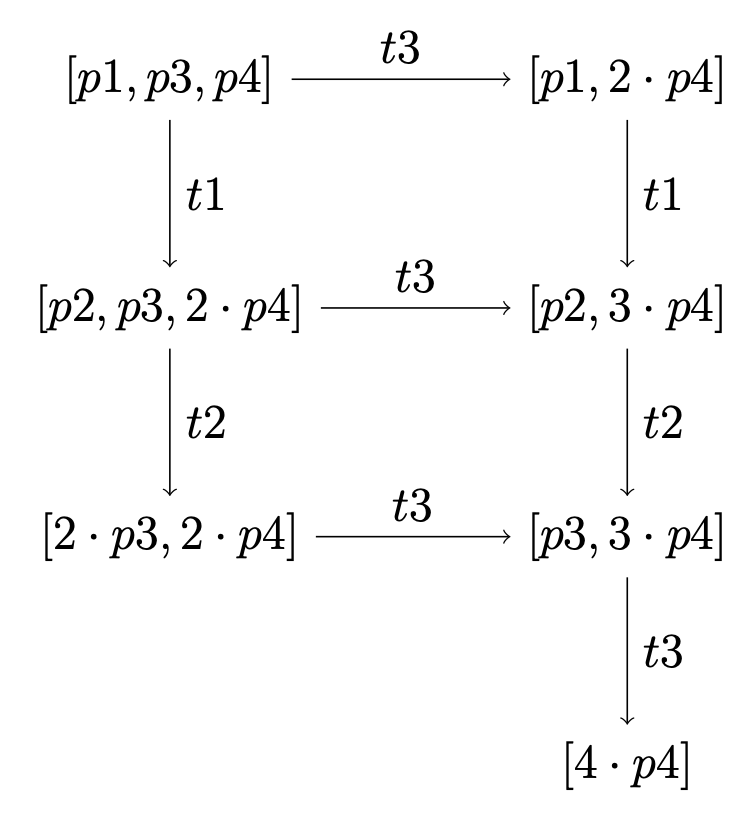
\includegraphics[width=0.5\textwidth]{images/exercises/petri_nets/reachability_graph.png}
        \caption{Reachability Graph of the Example Petri Net}
    \end{figure}
    \item The reachable terminal markings are the markings where no transitions are enabled. From the reachability graph, 
    we can see that the terminal marking is:
    \[ M_t: M(p_1) = 0, M(p_2) = 0, M(p_3) = 0, M(p_4) = 4 \]
    \item Yes, for example the marking \(M_0\) enables both transitions \(t_1\) and \(t_3\), leading to a non-deterministic choice between them.
\end{enumerate}